\documentclass[11pt, oneside]{article} 
\usepackage{geometry}
\geometry{letterpaper} 
\usepackage{graphicx}
	
\usepackage{amssymb}
\usepackage{amsmath}
\usepackage{parskip}
\usepackage{color}
\usepackage{hyperref}

\graphicspath{{/Users/telliott/Github/figures/}}
% \begin{center} \includegraphics [scale=0.4] {gauss3.png} \end{center}

\title{Pyramid and cone}
\date{}

\begin{document}
\maketitle
\Large

%[my-super-duper-separator]

We need a formula for the volume of a cone in order to find the volume of the sphere.  To find the cone's volume, let's start with something simpler, a pyramid with a square base.  

Below is a cube with all eight edges having length $s$.  Each of the six faces is a square with sides of length $s$ and area $s^2$.

Label the central point inside the solid as $P$.  Draw lines connecting each of the 8 external vertices to $P$, something like this. 
\begin{center}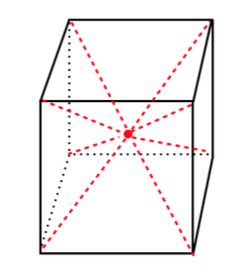
\includegraphics [scale=0.5] {cube_to_cone.png}\end{center}

Now we imagine slicing on planes that connect adjacent pairs of lines.  

You can't do this in real life by slicing up a single cube or rectangular solid, because the cuts to form one surface would ruin some of the other pieces.  The cuts must enter the solid at a corner and then pivot on a line ending at the exact center.

Perhaps you could do it with a \emph{light saber} since the beam comes to a point.

\begin{center}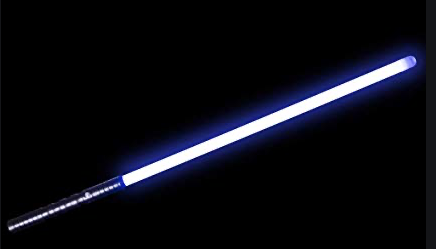
\includegraphics [scale=0.4] {light_saber.png}\end{center}

The result is 6 identical pieces (right square pyramids) looking something like this
\begin{center}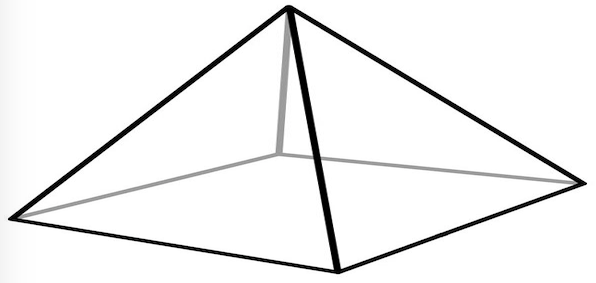
\includegraphics [scale=0.25] {sq_pyramid.png}\end{center}

The procedure described generates pyramids with height $s/2$ on a base of side length $s$.  I admit they are a little squat, but just hang on.

Since we started with a cube, and work from a central point, the six resulting solids are identical.  

You can either have six pieces come out exactly the same, as we've done, or start with an elongated base, so then two of the pieces will come out with equal base and height, but you can't do both at the same time by this construction.

Let the six identical pyramid volumes each be $V$.  Their sum is equal to the volume of the cube that we started with.

\[ 6V = s^3 \]
\[ V = \frac{1}{6} s^3  \]

The height $h = s/2$ so
\[ V = \frac{1}{3} \ hs^2 \]

This is the volume for each pyramid with base area $s^2$ and height $h = s/2$.  

By changing the area of the base or the height, you can alter the shapes obtained.  But all other constructions give at least two different types of pyramids, which means we can't simply divide by $6$ as we did.  This is, unfortunately, a fatal defect.

\subsection*{better way}

Here is a better way to slice a cube.

\begin{center}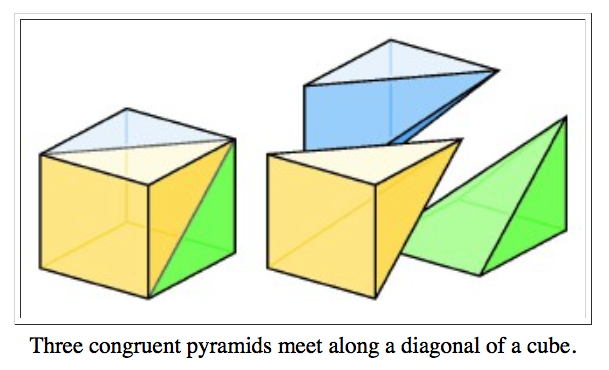
\includegraphics [scale=0.5] {pyramid_cube.png}\end{center}

When I first saw this, I thought it was a trick.  We have produced $3$ identical pyramids (they are called oblique because the apex is not in the center).

\url{http://www.math.brown.edu/~banchoff/Beyond3d/chapter2/section02.html}

Each pyramid has a square base, two vertical sides that were halves of the original sides, now cut along the diagonal.  The fourth and fifth sides slant down from the apex to the opposing sides.  Here are three views of one pyramid.

\begin{center}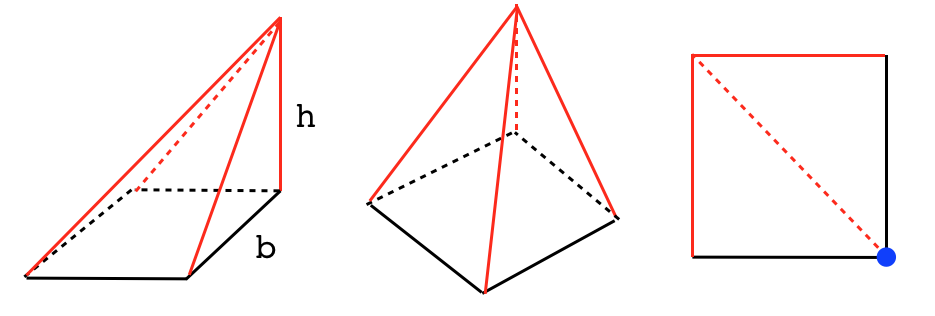
\includegraphics [scale=0.35] {pyr_proof1.png}\end{center}

On the right is a simple schematic way to draw pyramids, with perspective from the top.  The blue dot indicates the placement of the apex.

\subsection*{a cheese pyramid}

I found a fun method to do the demonstration easily and safely.  I was going to cut some wood on the table saw, but this is much better.

Get a thick piece of cheese and cut out a cube as large as you can make it and with everything squared as close as you can.

Then cut straight down on a diagonal all the way through the cube, resulting in two identical pieces.

If you now take each of the pieces and orient them with the new angled surface resulting from the cut facing up, you can then make another diagonal cut straight down for each (that cut has just been made, in the figure).  

\begin{center}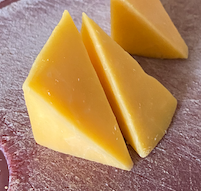
\includegraphics [scale=0.75] {cheese2.png}\end{center}

You can see that the second cut results in a large piece that has a square base (currently oriented to the left in the photo above), and a smaller piece with a triangular base, which is facing down and stays that way in the final arrangement.  

The two small pieces are mirror images that can be glued together into a single shape identical to each of the large pieces.

\begin{center}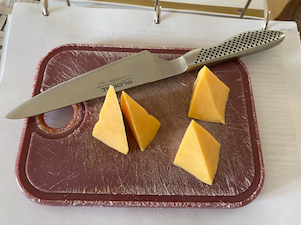
\includegraphics [scale=1.0] {cheese1.png}\end{center}

By this means we deconstruct the cube into three identical pyramids.  Good luck!  It is OK to eat the demonstration afterwards.

\subsection*{perspectives}

Our dissection proves that a pyramid with a square base and the apex placed directly above one of the vertices of the base has 

\[ V = \frac{1}{3} \ Bh \]

where $B$ is the area of the base and $h$ is the height.  

Here is that sketch again.  The vertex lies directly above the edge labeled $h$.

\begin{center}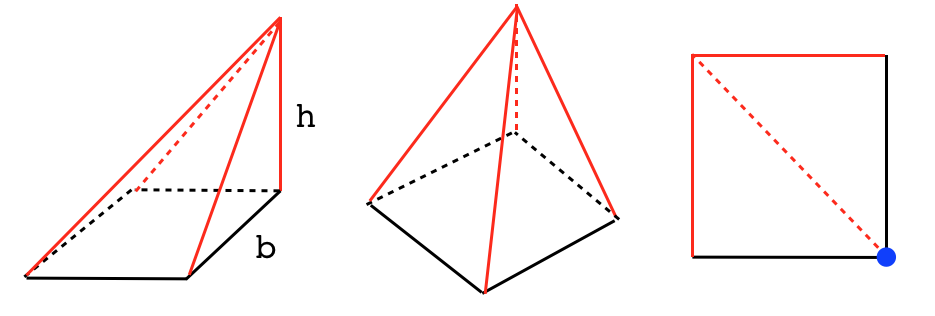
\includegraphics [scale=0.35] {pyr_proof1.png}\end{center}

Solid lines outline the base, and the color of the line indicates whether that side meets the plane of the base in a right angle (black) or on a slant (red).  Because of the right angle, the solid black line hides the diagonal along the side up to the vertex.

The other kind of diagonal (not overlying a side of the base) is shown as a dotted line. 

\subsection*{moving the apex}

It is natural to look at other shapes for the base, and other placements for the apex.  This is a right square pyramid.  

\begin{center}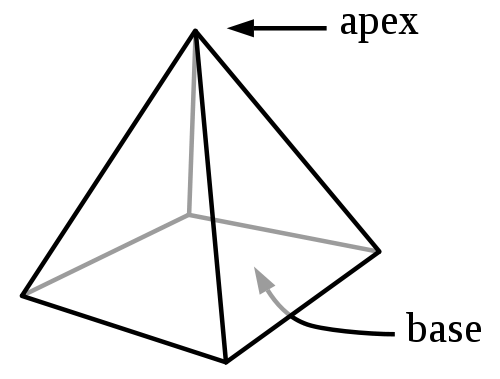
\includegraphics [scale=0.25] {volume_cone_rtpyr.png}\end{center}

The apex lies above the center of the base.  Here is the perspective view (below, left panel).

\begin{center}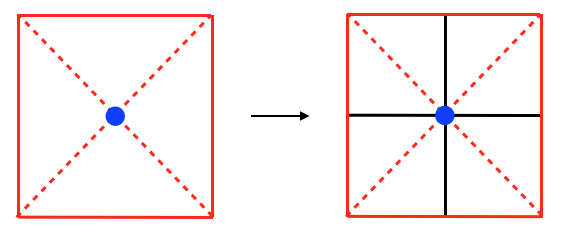
\includegraphics [scale=0.4] {pyr_proof2.png}\end{center}

The point is that the right pyramid can be cut into four identical cheese pyramids (right panel).  Therefore the volume of each is one-fourth, and so is the base.  

We have proved the formula works for a right pyramid.

The next question is how to prove that we can put the apex anywhere and still have the same volume.

\begin{center}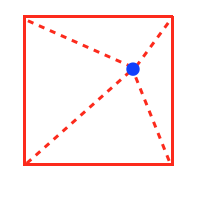
\includegraphics [scale=0.5] {pyr_proof3.png}\end{center}

At the moment, I know how to turn that into a regular rectangle, but not into a square:

\begin{center}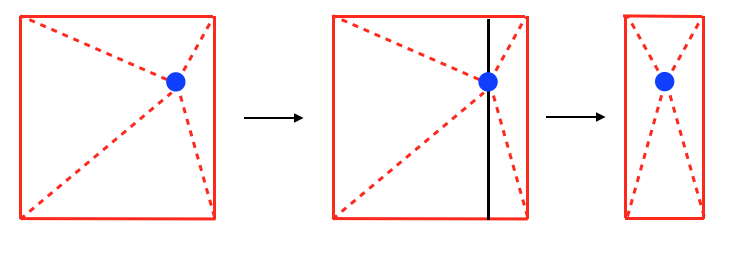
\includegraphics [scale=0.4] {pyr_proof5.png}\end{center}

\subsection*{triangular pyramid}
It is also easy to show that a triangular base with the apex directly above a vertex obeys the  volume rule.

\begin{center}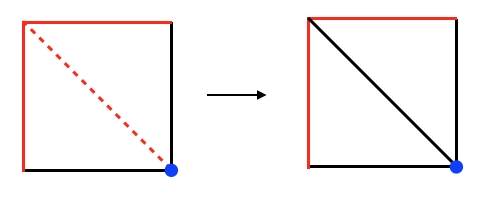
\includegraphics [scale=0.4] {pyr_proof4.png}\end{center}

We have two identical triangular pyramids, and half the base for each one.

If we had rectangles, by using them we could produce a triangular base of any shape.  If necessary, we can put two together to form an isosceles base.

In the figure below, on the left, is a view of that same pyramid cut from cheese, drawn with the height extended to make it easier to see.

\begin{center}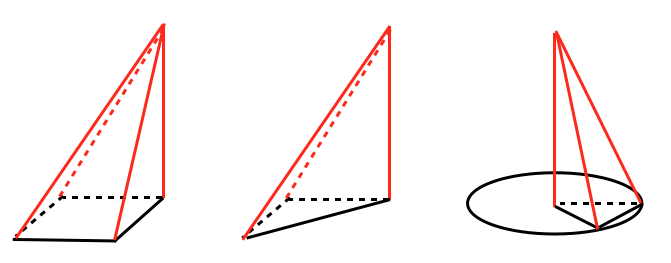
\includegraphics [scale=0.4] {pyr_proof7.png}\end{center}

In the middle is one of two identical halves constructed by bisecting the square pyramid.  Its base has become triangular.  Clearly it is still the case that $V = Bh/3$, since halving the base gave two identical shapes each with half the volume.

On the right side, we have a triangular pyramid inscribed in a cone.  The volume of the cone will be the summed volume of the inscribed pyramids, whose bases, as Archimedes showed, become the area of a circle.

Both the triangular pyramid cut from cheese and the shape we need on the right have two vertical sides, at right angles to the plane of the base.  The  difference between them is that one vertex on the base is a right angle, whereas for the one we need, the angles of the base of the pyramid on the right depend on the size of the slice.

We are close, but not there yet.

Euclid proves the volume formula in book XII of the \emph{Elements}.  However, the proofs are much too long for us, and ultimately, this problem has a trivial solution in our first bit of calculus.

\subsection*{cone}

A pyramid is not a cone.  But we believe, based on these ideas, that the volume is independent of the shape of the base.  It just depends on the area.  

There is another hand-waving argument from the age before calculus.  It is called Cavalieri's principle, also the \emph{method of indivisibles}, or the stack of quarters argument.
\begin{center}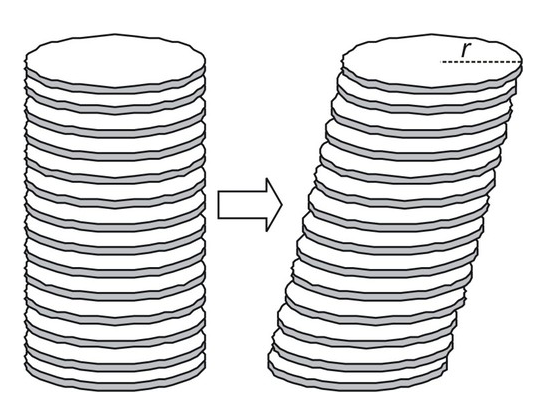
\includegraphics [scale=0.2] {volume_cone_quarters.png}\end{center}

\url{https://en.wikipedia.org/wiki/Cavalieri's_principle}

Knowing basic calculus allows us to see easily where the factor of one-third comes from in the formula for the volume of a pyramid or a cone.  It comes from integrating $x^2 \ dx$ and obtaining $x^3/3$.  Get there we will, young padawan.  If you want to peek ahead, it is \hyperref[sec:vol_cone_calculus]{\textbf{here}}.

\subsection*{algebraic derivation of the constant 1/3 for a cone}

I found an algebraic derivation on the web at 

\url{https://web.maths.unsw.edu.au/~mikeh/webpapers/paper47.pdf}

Let us assume for this proof that the volume of a cone is proportional to both the area of the base and the height:  $V = cAh$;  our objective is to find the constant of proportionality.

It takes a bit of algebra to see, but gives the value for the proportionality constant as $1/3$.

Consider a conical frustum, a cone with the top lopped off.  

\begin{center} 
\includegraphics [scale=0.3] {conical_frustum.png} \end{center}

Suppose the area of the base is $A$ and the height of the frustum is $h$.  

Calculate the volume of the frustum as the difference between that of a larger cone with base $A$ and height $h + e$ (e for extra), and that of a small cone (the part cut off to form the frustum) with base area $a$ and height $e$.

\[ V = cA(e + h) - cae \]

Now, the area of the base of a cone is $\pi$ times the radius squared, and the radius is proportional to the height (depending on how sharply the side slants).  Hence
\[ a = \pi r_2^2 = ke^2 \]

The area of the small base is proportional to the height squared, and so is the large one, with the same proportionality constant:
\[ A = k(e + h)^2 \]
thus
\[ \frac{a}{A} = \frac{ke^2}{k(e + h)^2} \]
\[ \frac{\sqrt{a}}{\sqrt{A}} = \frac{e}{e + h} \]

Let us manipulate this expression to find $e$ in terms of $h$.  It just requires a bit of facility with square roots:

\[ \frac{\sqrt{A}}{\sqrt{a}} = \frac{e + h}{e} = 1 + \frac{h}{e} \]
\[ \frac{h}{e} = \frac{\sqrt{A}}{\sqrt{a}} - 1 \]
\[ = \frac{\sqrt{A} - \sqrt{a}}{\sqrt{a}} \]
\[ e = \frac{\sqrt{a}}{\sqrt{A} - \sqrt{a}} \cdot h \]

And then
\[ e + h = \ [ \  \frac{\sqrt{a}}{\sqrt{A} - \sqrt{a}} + 1 \ ] \ h =\frac{\sqrt{A}}{\sqrt{A} - \sqrt{a}} \cdot h \]

Substituting into what we had above for the volume:
\[ V = cA(e+h) - cae \]
\[ = cA \ [ \frac{\sqrt{A}}{\sqrt{A} - \sqrt{a}} \cdot h \ ] - ca \ [ \frac{\sqrt{a}}{\sqrt{A} - \sqrt{a}}  \cdot h \ ] \]
\[ = c \ [ \   \frac{A \sqrt{A} - a \sqrt{a}}{\sqrt{A} - \sqrt{a}} \ ] h \]

This really looks like a mess.  

But suppose we let $m =  \sqrt{A}$ and $n =  \sqrt{a}$ so
\[ \sqrt{A} - \sqrt{a} = m - n \]
then the numerator above is really just $m^3 - n^3$.    

We can factor that, we get 
\[ m^3 - n^3 = (m-n)(m^2 + mn + n^2) \]
which you can confirm by multiplying back out.  So the first term $(m-n)$ cancels the denominator.  We now have:

\[ V = c (m^2 + mn + n^2) h \]
\[ V = c (A + \sqrt{A} \sqrt{a} + a) h \]

Here's the point:  consider what happens as $a$ gets larger and closer to $A$.

We say:  let $a \rightarrow A$.

The expression in parentheses becomes $3A$.  Hence:
\[ V = c(3A)h \]
But if $a = A$, the frustum has become a cylinder, whose volume we know.  It is equal to $Ah$. 
\[ V = c(3A)h = Ah \]

Therefore $c = 1/3$.

$\square$

\end{document}